\begin{filecontents}{preliminary.sty}
\ProvidesPackage{preliminary}
%\DeclareOption{draft}{%
  \AtBeginDocument{%
    \renewcommand\maketitlehookc
\ProcessOptions
\RequirePackage{titling}
\endinput
\end{filecontents}

\documentclass[12pt, a4paper]{article}
\usepackage{setspace}
\usepackage{ragged2e}
\usepackage[centertags,reqno]{amsmath}
\usepackage{amssymb}
\usepackage{graphics,subfigure}
\usepackage[dvips]{graphicx}
\usepackage[dvipsnames]{xcolor}
\usepackage[hidelinks]{hyperref}
\usepackage{appendix}
\usepackage{natbib}
\usepackage{verbatim,color}
\usepackage{pdflscape}
\usepackage[showframe=false]{geometry}
\usepackage{changepage}
\usepackage{xcolor}
\usepackage{eurosym}
\usepackage{textcomp}
\usepackage[open,openlevel=1]{bookmark}
\usepackage{multirow}
\usepackage{caption}
\usepackage{hyphenat}
\newcommand{\mybox}[2]{{\color{#1}\fbox{\normalcolor#2}}}
\doublespacing

% Exception to hyphenation
\hyphenation{par-ti-ci-pants}
\hyphenation{par-ti-ci-pant}
\hyphenation{Hy-po-the-sis}
\hyphenation{ex-pe-ri-ment}
\hyphenation{ex-pe-ri-ments}

% Allows bigger tables to be scaled down
\usepackage{adjustbox}

%From my paper with Raymond
\usepackage{tabularx,calc}
\usepackage{dcolumn}                    % Aligns tables on the decimal point
\newcolumntype{d}[1]{D{.}{.}{#1}}       %       Aligns on dot
\newcolumntype{.}{D{.}{.}{3.5}}         %       Somehow it works better
\newcolumntype{C}{@{\extracolsep{.6cm}}c@{\extracolsep{0pt}}}
\usepackage{threeparttable}
\usepackage{siunitx,booktabs}
\sisetup{
    detect-all,
    round-integer-to-decimal = true,
    group-digits             = true,
    group-minimum-digits     = 4,
    group-separator          = {\,},
    table-align-text-pre     = false,
    table-align-text-post    = false,
    input-signs              = + -,
    input-symbols            = {*} {**} {***},
    input-open-uncertainty   = ,
    input-close-uncertainty  = ,
    retain-explicit-plus
}

% Commands to name appendices Appendix A, Appendix B, etc.
\makeatletter
%% The "\@seccntformat" command is an auxiliary command
%% (see pp. 26f. of 'The LaTeX Companion,' 2nd. ed.)
\def\@seccntformat#1{\@ifundefined{#1@cntformat}%
   {\csname the#1\endcsname\quad}  % default
   {\csname #1@cntformat\endcsname}% enable individual control
}
\let\oldappendix\appendix %% save current definition of \appendix
\renewcommand\appendix{%
    \oldappendix
    \newcommand{\section@cntformat}{\appendixname~\thesection\quad}
}

%Adds text specifying it is a preliminary version
\usepackage{preliminary}

\title{Eliciting Minimum Acceptable Probabilities \\
\Large Pre-Analysis Plan}
\author{Martin Strobel  \and Maria Polipciuc\thanks{Maastricht University. Email: \url{m.polipciuc@maastrichtuniversity.nl}. We thank Elias Tsakas for valuable comments.}}
\date{\today	\vspace{1cm}}
\titlepage


\begin{document}
\begin{titlepage}
\clearpage\maketitle
\thispagestyle{empty}

\end{titlepage}
\section{Main page description (public)}
\large \textcolor{RoyalBlue}{\textbf{Interventions}}

\normalsize \noindent \textcolor{NavyBlue}{\textbf{Intervention(s)}}

We compare minimum acceptable probabilities (MAPs) for which a participant prefers a binary lottery to a sure payoff across treatments within individual.
Individuals have to decide in randomized order in three scenarios (treatments).
The treatments keep the sure payoff and the payoffs of the lottery fixed, but vary the distribution of the winning probability of the lottery.

\noindent \textcolor{NavyBlue}{\textbf{Trial Start Date}}

\textcolor{red}{Not applicable}

\noindent \textcolor{NavyBlue}{\textbf{Intervention Start Date}}

TBD

\noindent \textcolor{NavyBlue}{\textbf{Intervention End Date}}

TBD



\large \noindent \textcolor{RoyalBlue}{\textbf{Primary Outcomes}}

\normalsize \noindent \textcolor{NavyBlue}{\textbf{Primary Outcomes (end points)}}

MAPs

\noindent \textcolor{NavyBlue}{\textbf{Primary Outcomes (explanation)}}

The MAPs are elicited as thresholds for preferring a lottery to a sure payoff. 



\large \noindent \textcolor{RoyalBlue}{\textbf{Experimental Design}}

\normalsize \noindent \textcolor{NavyBlue}{\textbf{Experimental Design}}

We elicit MAPs in an online experiment in a lottery similar to the \textit{Decision Problem} in \cite{Bohnet2004}.
In this paper, \cite{Bohnet2004} find that participants require a premium for being willing to trust someone compared to taking an equally risky bet with the same payoff externalities for an uninvolved person.
They attribute this premium to betrayal aversion---an anticipatory disutility from exposing oneself to the risk of being betrayed.

As \cite{Li2020a} note, this attribution rests on the assumption that participants are rational expected utility maximizers.
Should participants not be rational expected utility maximizers, there are several possible confounding explanations for the premium found by \cite{Bohnet2004} and subsequent studies, such as ``ambiguity attitudes, complexity, different beliefs, and dynamic optimization'' \citep[p.~275]{Li2020a}.

In this study, we test experimentally what the contribution of one such confounding explanation is to this premium.
Specifically, we test whether participants' declared MAPs change as a result of the underlying distribution from which the probability of success of the gamble is drawn.
We exogenously manipulate participants' beliefs about this distribution by varying the different objective distributions from which the probability of success $p^*$ is drawn.
We then compare the resulting MAPs across treatments.

\noindent \textcolor{NavyBlue}{\textbf{Experimental Design Details}}

See the pre-analyis plan

\noindent \textcolor{NavyBlue}{\textbf{Randomization Method}}

Computer

\noindent \textcolor{NavyBlue}{\textbf{Randomization Unit}}

Individual

\noindent \textcolor{NavyBlue}{\textbf{Was the treatment clustered?}}

No

\noindent \textcolor{NavyBlue}{\textbf{Planned Number of Observations}}

\textcolor{red}{420}
    
\noindent \textcolor{NavyBlue}{\textbf{Was IRB approval obtained (only for ``In Development" and ``On-going" trials)?}} If so, also

        IRB Name
        
        IRB Approval Date
        
        IRB Approval Number
        
\textcolor{red}{No, but the experiment has been approved in a BEELab proposal meeting at Maastricht University.}





\section{Introduction}
The Minimum Acceptable Probability (MAP) is a threshold value elicited through a procedure similar to a Becker-DeGroot-Marschak mechanism (expressed as the probability or as the number of favorable outcomes) for preferring to trust someone over accepting a sure payoff.

The concept was introduced by \cite{Bohnet2004} and it has been used—with slight variations—to elicit a determinant of trust, betrayal aversion, in a difference-in-difference design.
As \cite{Li2020a} show, if participants are not rational expected utility maximizers, there are several other confounding explanations for the premium.

This paper investigates whether the MAP is influenced by a participant’s belief about the distribution from which the chance of a favorable outcome is drawn. 
We remove the social and strategic aspects of a trusting decision, and study the MAP for accepting a risky lottery.
The treatments vary the distribution from which the chance of the favorable outcome is drawn, thus manipulating participants’ expectations about the lottery’s winning chances.


Below we present the sample selection procedure, the experimental design, and the empirical strategy.



\section{Research Strategy}
This project will collect experimental data on an online platform dedicated to academic research (Prolific) in May 2021. Participants will be exposed to three treatments sequentially, in randomized order.
In each of the treatments, participants have to state the MAP (minimum acceptable probability) for which they prefer a lottery over a sure payment.
%This is a version of \citeauthor{Bohnet2004}'s (\citeyear{Bohnet2004}) \textit{Decision Problem} (p. 469).
%The treatments differ in the underlying distribution from which the lottery is drawn.
%Given the complexity of the task, we will recruit participants with completed higher education, to increase the chances that task comprehension is not an issue.

The pre-analysis plan will be registered at the AEA RCT registry before the start of the data collection.


\subsection{Recruitment}
Participants are registered users on the online platform Prolific.
This platform is tailored for academic research, and gathers demographics about registered users.
We will send an invitation to the experiment only to participants who have completed higher education to increase the chances that task comprehension is not an issue.
Our sample consists of residents of the United Kingdom.



\section{Design}
The study consists of three parts.
The first part describes the task and asks comprehension questions.
This part pays a fixed payoff.
Only those who answer the comprehension questions correctly are directed to the second part, which is incentivized.
After this, those who complete the second part go through a survey (the third part), which is unincentivized.
Uncertainty is resolved at the very end, when participants are informed about their payoff for the second part.

As mentioned above, participants in the experiment are asked to state their MAP in a \textit{Decision Problem}: what is their MAP for taking a gamble rather than accepting a sure payoff?
The experiment uses a within-subject design.
The complete instructions are available in Appendix \textcolor{red}{XYZ}.

Below we present the main task in more detail.

\subsection{Explanation of the main task in Part 1}
See the document `Explanation.pdf'.

%\subsection{Comprehension questions}
%TBD

\subsection{Main task in Part 2}
In each treatment, the subjects are faced with a different distribution of the possible states of the world.
Each state of the world is represented by a wheel of fortune with 15 sectors.
Sectors are either dark blue (worth the high payoff of \pounds4) or light blue (worth the low payoff of \pounds1).
Each of the three treatments consists of 32 different wheels, which can be ordered by the overall expected value over all wheels in the treatment.
We call the three treatments: the Good (the treatment with the highest expected value over all 32 wheels, which is left-skewed), the Bad (the treatment with the lowest expected value over all 32 wheels, which is right-skewed), and the Uniform (the expected value is in-between the ones in the other treatments, and the distribution of risk is uniform).
The Bad and the Uniform distribution were chosen to reflect potential distributions imagined by participants in \cite{Bohnet2004} and \cite{Bohnet2008} in the Trust Game and in the Decision Problem, respectively.
Specifically, the Bad distribution has an expected probability of a blue sector over all 32 wheels of 0.2895, close to $p^*$ in the Trust Game.
The Uniform distribution is plausibly what participants expected to face in the Decision Problem.

Payoffs are determined by a two-stage lottery with objective probabilities.
In Stage 1, one of the 32 wheels is randomly drawn.
In Stage 2, the number of blue sectors in the randomly selected wheel is compared with the participant's MAP.
Should this number be equal to or exceed her MAP, the participant spins the virtual wheel for her payoff.
Should the number be lower than her MAP, the wheel is not spun, and the participant receives the intermediate safe payoff of \pounds2.

After having answered the comprehension questions in Part 1 correctly, participants see a picture like the one in Figures \ref{fig:thegood}, \ref{fig:thebad}, \ref{fig:theuniform}, with the following text:

\begin{figure}[h!]
  \centering
 {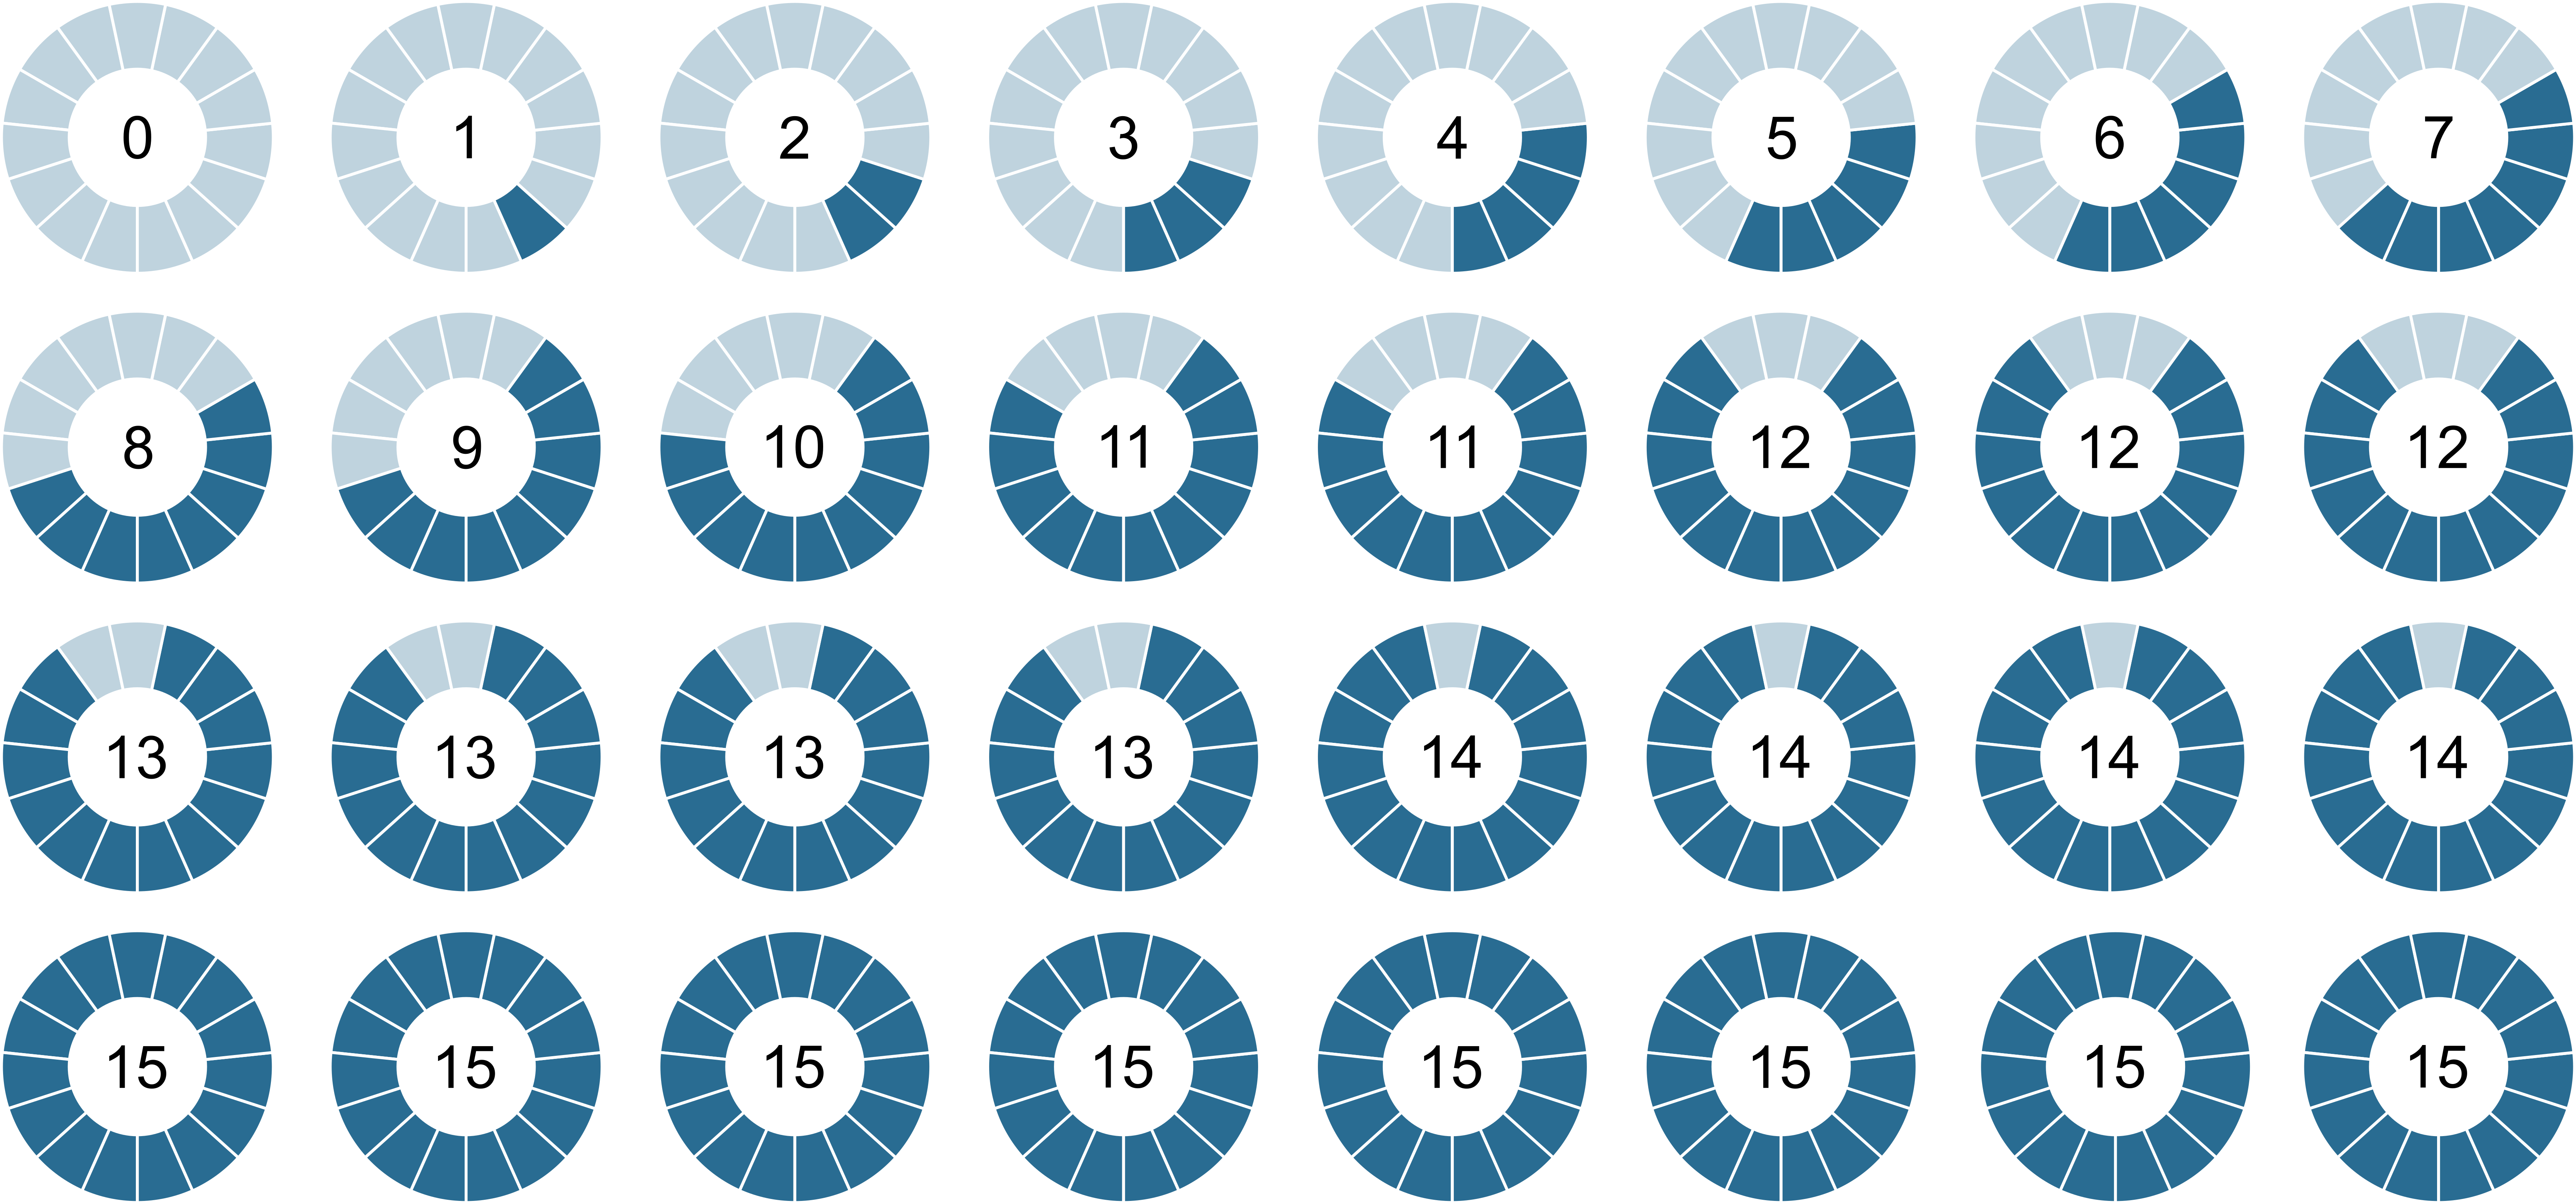
\includegraphics[width=0.95\linewidth]{Left_15.png}}
  \caption{Left-skewed distribution (`The Good')}
  \label{fig:thegood}
\end{figure}


\begin{figure}[h!]
  \centering
 {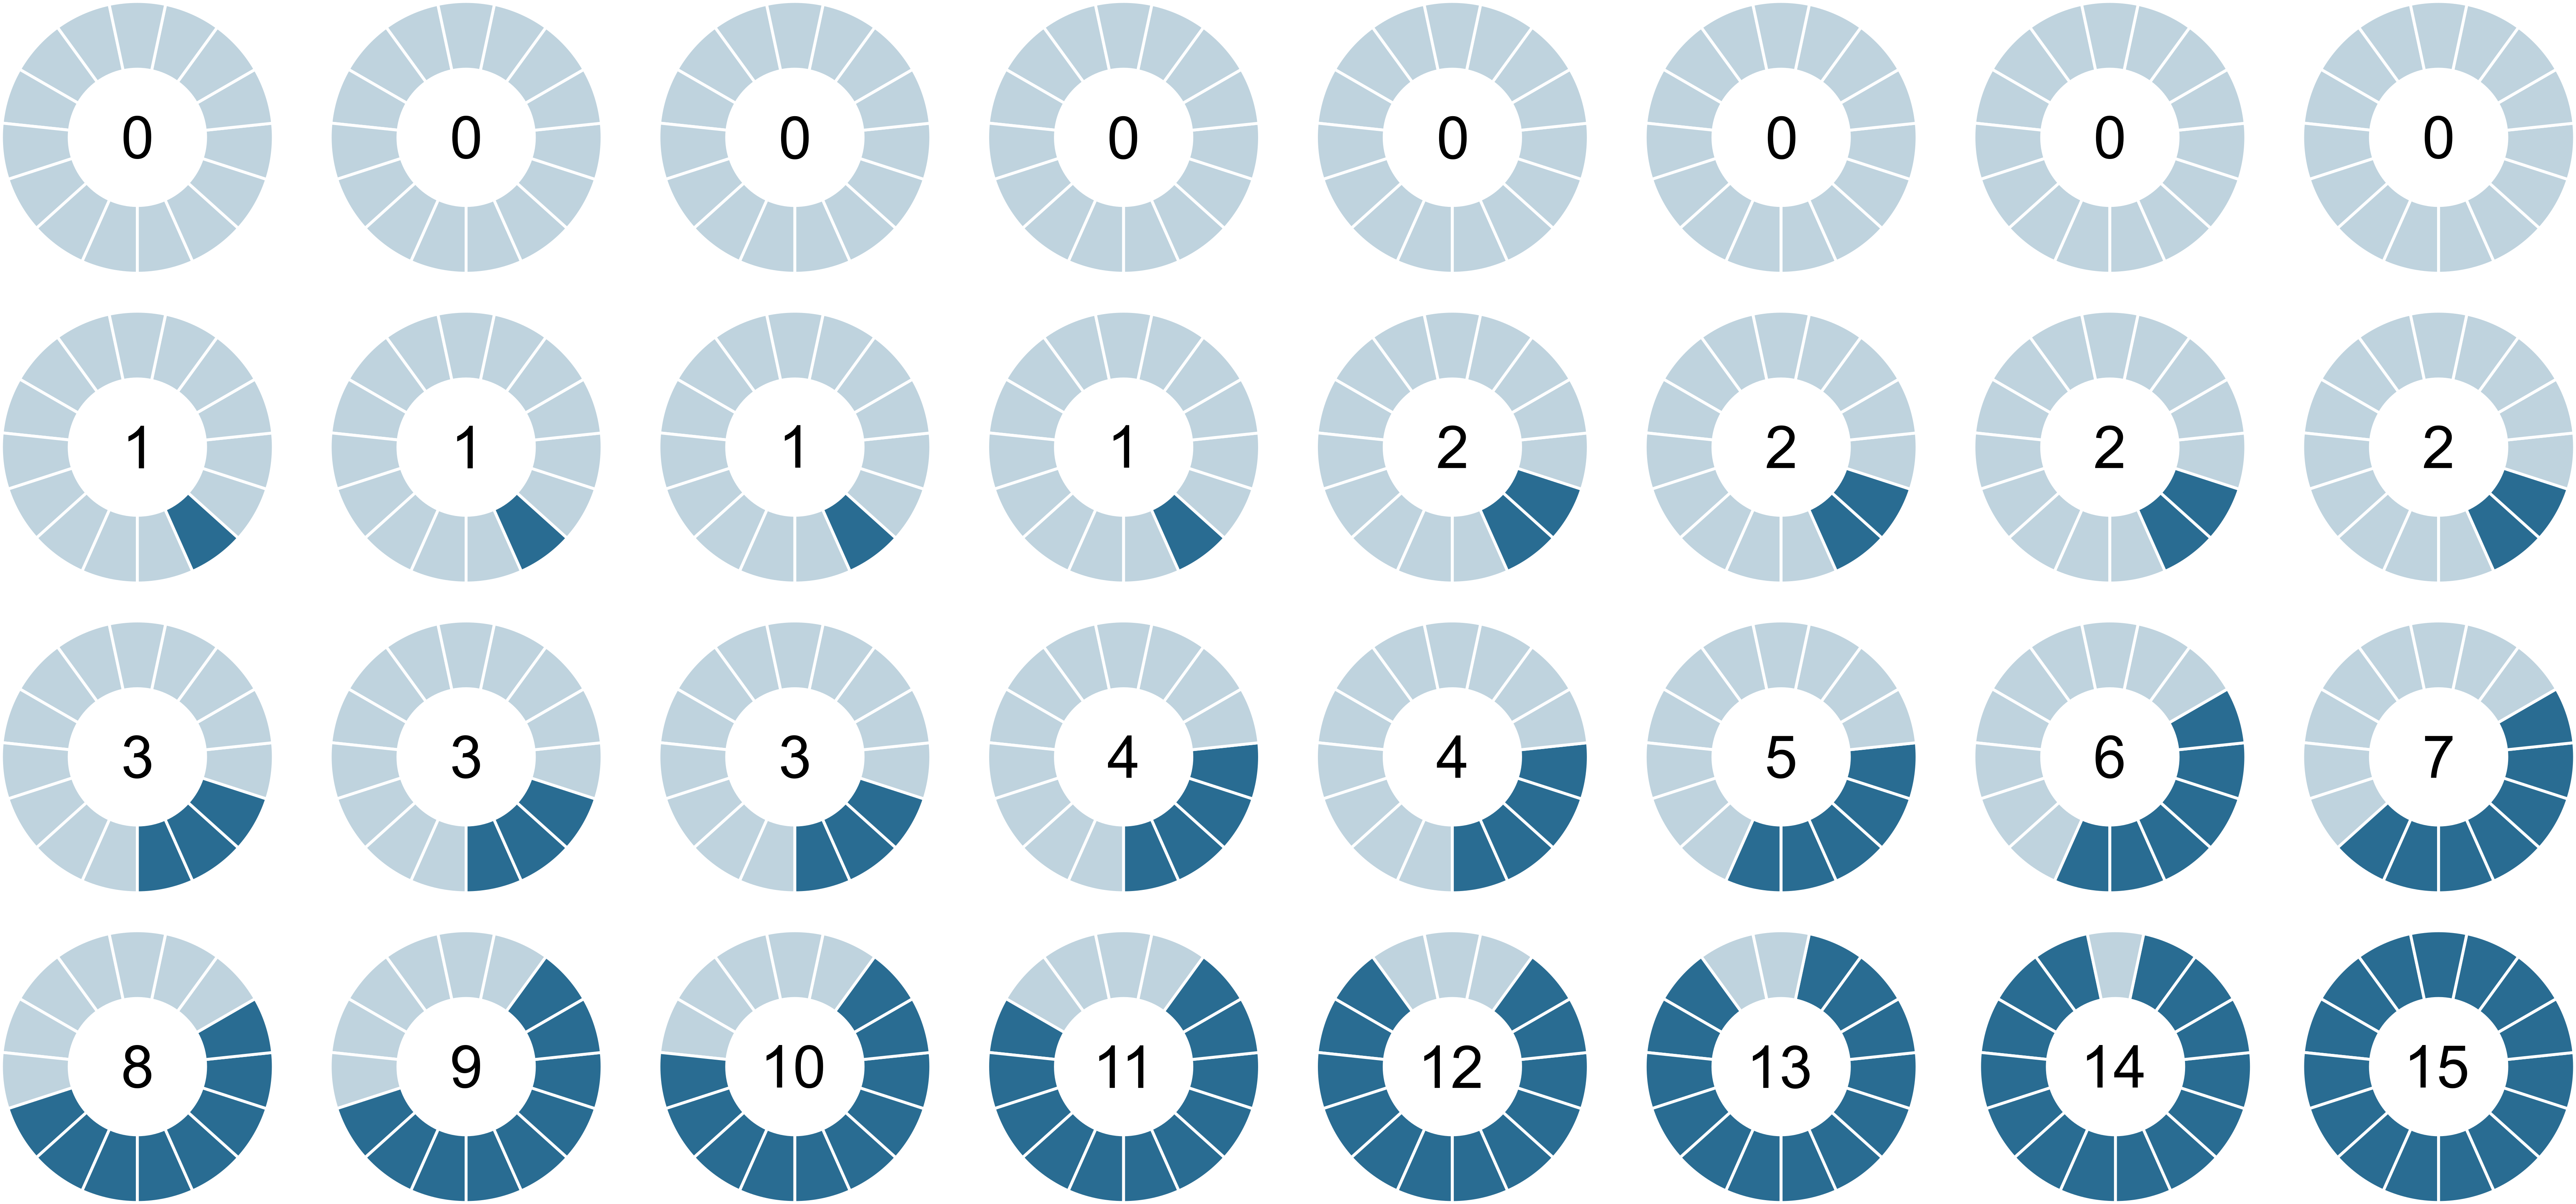
\includegraphics[width=0.95\linewidth]{Right_15.png}}
  \caption{Right-skewed distribution (`The Bad')}
  \label{fig:thebad}
\end{figure}


\begin{figure}[h!]
  \centering
 {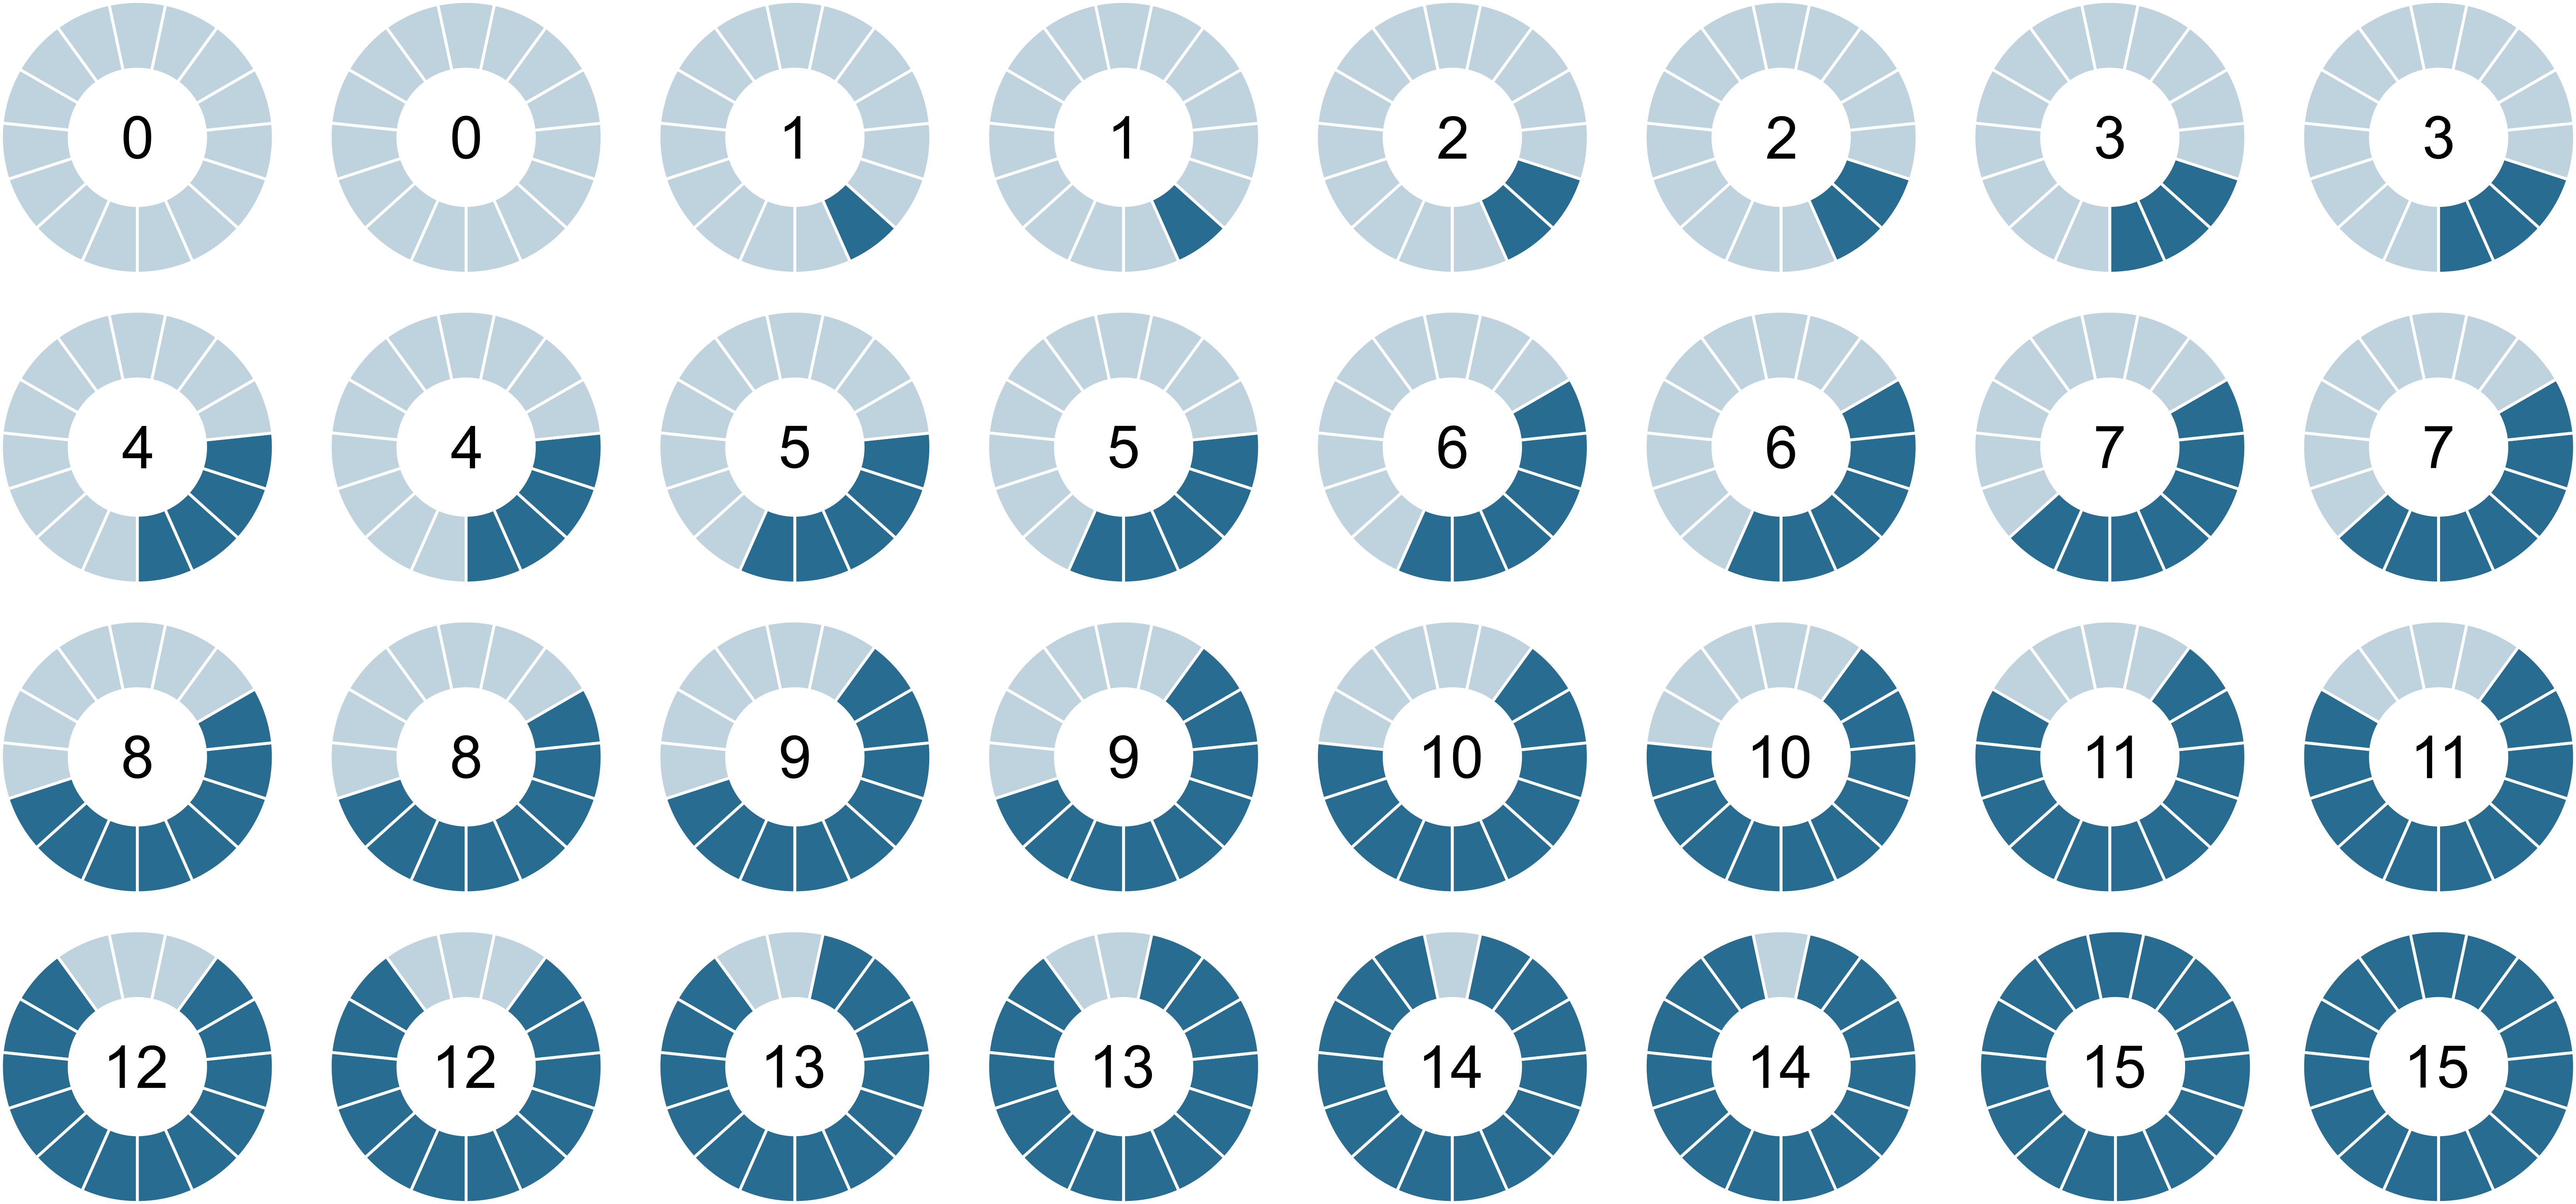
\includegraphics[width=0.95\linewidth]{Uniform_15.png}}
  \caption{Uniform distribution (`The Uniform')}
  \label{fig:theuniform}
\end{figure}

\textit{Consider the wheels above. Which wheels do you prefer to SPIN for your bonus?
Please enter an integer between 0 and 15.}

\textit{I prefer to SPIN wheels which have at least ... dark blue sectors.}

\textit{If the randomly selected wheel has fewer than ... dark blue sectors, I DON'T SPIN it.
My bonus is \pounds2.}

\textit{If the randomly selected wheel has ... or more dark blue sectors, I SPIN it.
My bonus is}
\begin{itemize}
\item \textit{\pounds1 if the selected wheel lands on a light blue sector, and}
\item \textit{\pounds4 if it lands on a dark blue sector.}
\end{itemize}

\subsection{Survey questions in Part 2}
Participants answer the following type of questions:
\begin{itemize}
\item an adapted cognitive reflection test \citep{Frederick2005,Thomson2016};
\item a general risk taking question \citep{Dohmen2011};
\item a question about their aspiration level for earnings from participating in a survey;
\item a couple of questions to check their anchoring susceptibility, from which an anchoring score can be computed \citep{Cheek2017};
\item a set of questions about their optimism/pessimism, the revised Life Orientation Test \citep{Scheier1994};
\item a brief sensation seeking scale, BSSS-4 \citep{Stephenson2003}.
\end{itemize}

Additional information will be requested from Prolific, who can provide data on participants' age, gender, and investment behavior.




\section{Empirical Strategy}
Should participants be expected utility maximizers, their MAPs should not differ between the three treatments.
This would be in line with what \cite{Bohnet2004,Bohnet2008} assume.

In their Appendix A, \cite{Li2020a} show by means of a numerical example that if participants are not expected utility maximizers, ambiguity aversion alone could generate the pattern attributed to betrayal aversion.
Since there is evidence that attitudes towards complex risks and attitudes towards ambiguity are correlated \citep{Armantier2016}, we redo their numerical exercise for our three distributions: the Good, the Bad and the Uniform in \textcolor{red}{Appendix XYZ}.
For this calculation we thus assume that participants view the tasks as complex risky situations---and this underlies their inverse S-shaped probability weighting.

This calculation leads to the following hypotheses.\footnote{
For details, see \textcolor{red}{Appendix XYZ}.
}


\subsection{Hypotheses}
\subsubsection{Main hypotheses}
\noindent \textbf{Hypothesis 1} \quad \textit{The MAP in the Good treatment (more mass on high values of $p^*$) is lower than the MAP in the Bad treatment (more mass on low values of $p^*$).}

\noindent \textbf{Hypothesis 2} \quad \textit{The MAP in the Good treatment (more mass on high values of $p^*$) is lower than the MAP in the Uniform treatment (a uniform distribution over $p^*$).}

\noindent \textbf{Hypothesis 3} \quad \textit{The MAP in the Bad treatment (more mass on low values of $p^*$) is higher than the MAP in the Uniform treatment (a uniform distribution over $p^*$).}

\subsubsection{Heterogeneity}
Since the MAP is a way to gauge (complex) risk aversion, we expect that in the same treatment females state higher MAPs than males on average.

\noindent \textbf{Hypothesis 4} \quad \textit{Within each treatment, females require higher MAPs on average than males.}

Our treatments vary the objective distribution of the winning probability.
How subjects process these probabilities might depend on things like (i) their optimism/pessimism \textcolor{red}{etc}.
These heterogeneity analyses will be based on subsamples resulting from answers to the post-experimental survey.\footnote{
Gender is among the demographics which we can obtain from Prolific.
}

\noindent \textbf{Hypothesis 5} \quad \textit{Within each treatment, more optimistic individuals require lower MAPs on average than pessimistic individuals.}

%\textcolor{red}{Maybe a question on taking risks? Concerns with fairness? External reference point for earnings e.g. how much should a 45-minute survey pay for you to be willing to take it (if it pays a fixed amount)?--> if international sample, allow them to select currency}



\subsection{Specifications and Analysis}
We present the OLS regressions which will be used to test the hypotheses.
Additionally, we will also run non-parametric Mann-Whitney U tests and \textcolor{red}{Friedman tests, to check whether the MAPs in all treatments are from the same distribution.}

The main hypotheses (1--3) will be tested using the following regression:
\begin{equation} \label{eq:1}
MAP_i = \beta + \beta_L L + \beta_R R + \epsilon_i
\end{equation}

\noindent where $MAP_i$ is the MAP chosen by participant $i$, $L$ is an indicator which takes the value of 1 if the decision was made in the Good treatment, $R$ is an indicator which is 1 if the decision was made in the Bad treatment and $\epsilon_i$ is a random error term.
Standard errors in the estimation will be clustered at the individual level.

For heterogeneity analyses, we will interact all terms in equation (\ref{eq:1}) with an indicator variable corresponding to each specific hypothesis.
For instance, for Hypothesis 5, all terms will be interacted with indicator variable $F_i$, which takes the value 1 if the participant is female:
\begin{equation} \label{eq:2}
MAP_i = \beta + \beta^F F_i + \beta_L L + \beta_L^F L F_i + \beta_R R + \beta_R^F R F_i + \epsilon_i
\end{equation}

The formal statements of the hypotheses are in the Appendix.

\clearpage
\pagebreak
\bibliographystyle{apalike}
\bibliography{Communities}

\clearpage
\pagebreak

\appendix
\section{Hypothesis Testing}
\label{section:appendixa}
\setcounter{figure}{0}
\setcounter{table}{0}
\renewcommand{\thefigure}{A.\arabic{figure}}
\renewcommand{\thetable}{A.\arabic{table}}

\subsection{Hypothesis 1}
$H0: \beta_L - \beta_R = 0 \\
H1: \beta_L - \beta_R < 0$

\subsection{Hypothesis 2}
$H0: \beta_L = 0 \\
H1: \beta_L < 0$

\subsection{Hypothesis 3}
$H0: \beta_R = 0 \\
H1: \beta_R > 0$

\subsection{Hypothesis 4}
Within each treatment:

\noindent $H0: \beta^F = 0 \\
H1: \beta^F > 0$

\noindent or

\noindent $H0: \beta^F + \beta_L^F = 0 \\
H1: \beta^F + \beta_L^F > 0$

\noindent or

\noindent $H0: \beta^F + \beta_R^F = 0 \\
H1: \beta^F + \beta_R^F > 0$

\subsection{Hypothesis 5}
Analogous to Hypothesis 4.

\end{document}